%!TeX root = ../Thesis.tex
\documentclass[../Thesis.tex]{subfiles}



\begin{document}


\begingroup
\clearpage% Manually insert \clearpage
\let\clearpage\relax% Remove \clearpage functionality
\vspace*{-2cm}% Insert needed vertical retraction



\chapter{Computing Fast and Reliable Gravitational Waveforms of Binary Neutron Star Merger Remnants}
\label{chapter:ComputingFastReliable}
\endgroup 





\chapterauthor{Paul J. Easter \\ Paul D. Lasky\\Andrew R. Casey\\Luciano Rezzolla\\Kentaro Takami}

\section*{Abstract}
	Gravitational waves have been detected from the inspiral of a binary neutron-star, GW170817, which allowed constraints to be placed on the neutron star equation of state. The equation of state can be further constrained if gravitational waves from a post-merger remnant are detected. Post-merger waveforms are currently generated by numerical-relativity simulations, which are computationally expensive. Here we introduce a hierarchical model trained on numerical-relativity simulations, which can generate reliable post-merger spectra in a fraction of a second. Our spectra have mean fitting factors of 0.95, which compares to a fitting factor of 0.93 between different numerical-relativity codes that simulate the same physical system. This method is the first step towards generating large template banks of spectra for use in post-merger detection and parameter estimation.

\section{Introduction}
    Gravitational waves have been  observed from the inspiral of binary neutron star merger GW170817~\cite{GW170817Detection}. This allowed limits to be placed on the neutron star tidal deformability ~(see~e.g.,~\cite{GW170817Detection,Annala2018,Radice2018,Most2018,De2018,GW170817Properties}). However, due to lack of detector sensitivity at high frequencies, the merger and post-merger signals were not detected~\cite{GW170817Properties,GW170817Postmerger1,GW170817Postmerger2}. Post-merger gravitational-waves from a binary neutron star merger could be detected with a signal-to-noise ratio of 5 at a distance of $\sim$25-40\,Mpc with Advanced LIGO at design sensitivity~\cite{Takami2014}.  The physics of the post-merger remnant is of particular interest as it probes the neutron star equation of state at significantly higher temperatures than the progenitor stars.\par 
    The detection and characterisation of a post-merger remnant is aided by a large bank of gravitational-wave strain waveforms. Generating such waveforms is currently computationally expensive, and there are only of order 100 in existence. In this work we make a step towards generating a large template bank of post-merger spectra by training a hierarchical model on a set of numerical-relativity spectra.\par    
    There has been significant research applied to the relationship between post-merger numerical-relativity simulations, the corresponding spectrum of the gravitational-wave strain, and the neutron star equation of state~(e.g.,~\cite{Stergioulas2011,Bauswein2012,Read2013,Hotokezaka2013,Takami2014,Bernuzzi2015,Takami2015,Clark2016postmerger,Rezzolla2016,Radice2017,Dietrich2017b,Radice2017a,Pietri2018,Dietrich2018,Dietrich2018a,Bose2018}). There are many degrees of freedom for each simulation, which include the neutron star system parameters, equation of state, and  simulation parameters (e.g., spacetime evolution formalism~\cite{Baiotti2017}, resolution), as well as parameters related to magnetic fields and neutrinos. We choose to use a set of numerical-relativity simulations that are homogeneous, eliminating unwanted variations between simulations with different parameters. To achieve this, we use a subset of 35 waveforms from Ref.~\cite{Rezzolla2016} consisting of identical simulation parameters with variations in the neutron star mass and equation of state only. To obtain consistent spectra, we select waveforms that have a fixed time-step and almost identical length. \par
    Ref.~\cite{Clark2016postmerger} showed that dimensional reduction of post-merger waveforms is possible by performing principal component analysis after aligning the maximum of each gravitational-wave strain spectra in the frequency domain (see also \cite{Bose2018}). We use a similar method of frequency shifting in our model. We introduce a hierarchical model that trains on existing numerical-relativity post-merger simulations, and can produce new, accurate spectra in a fraction of a second. This is the first step towards making large template banks of post-merger spectra suitable for detection and parameter estimation which could compliment existing unmodelled searches for post-merger remnants~\cite{GW170817Properties,Klimenko2016,Chatziioannou2017}. \par
\begin{figure*}
    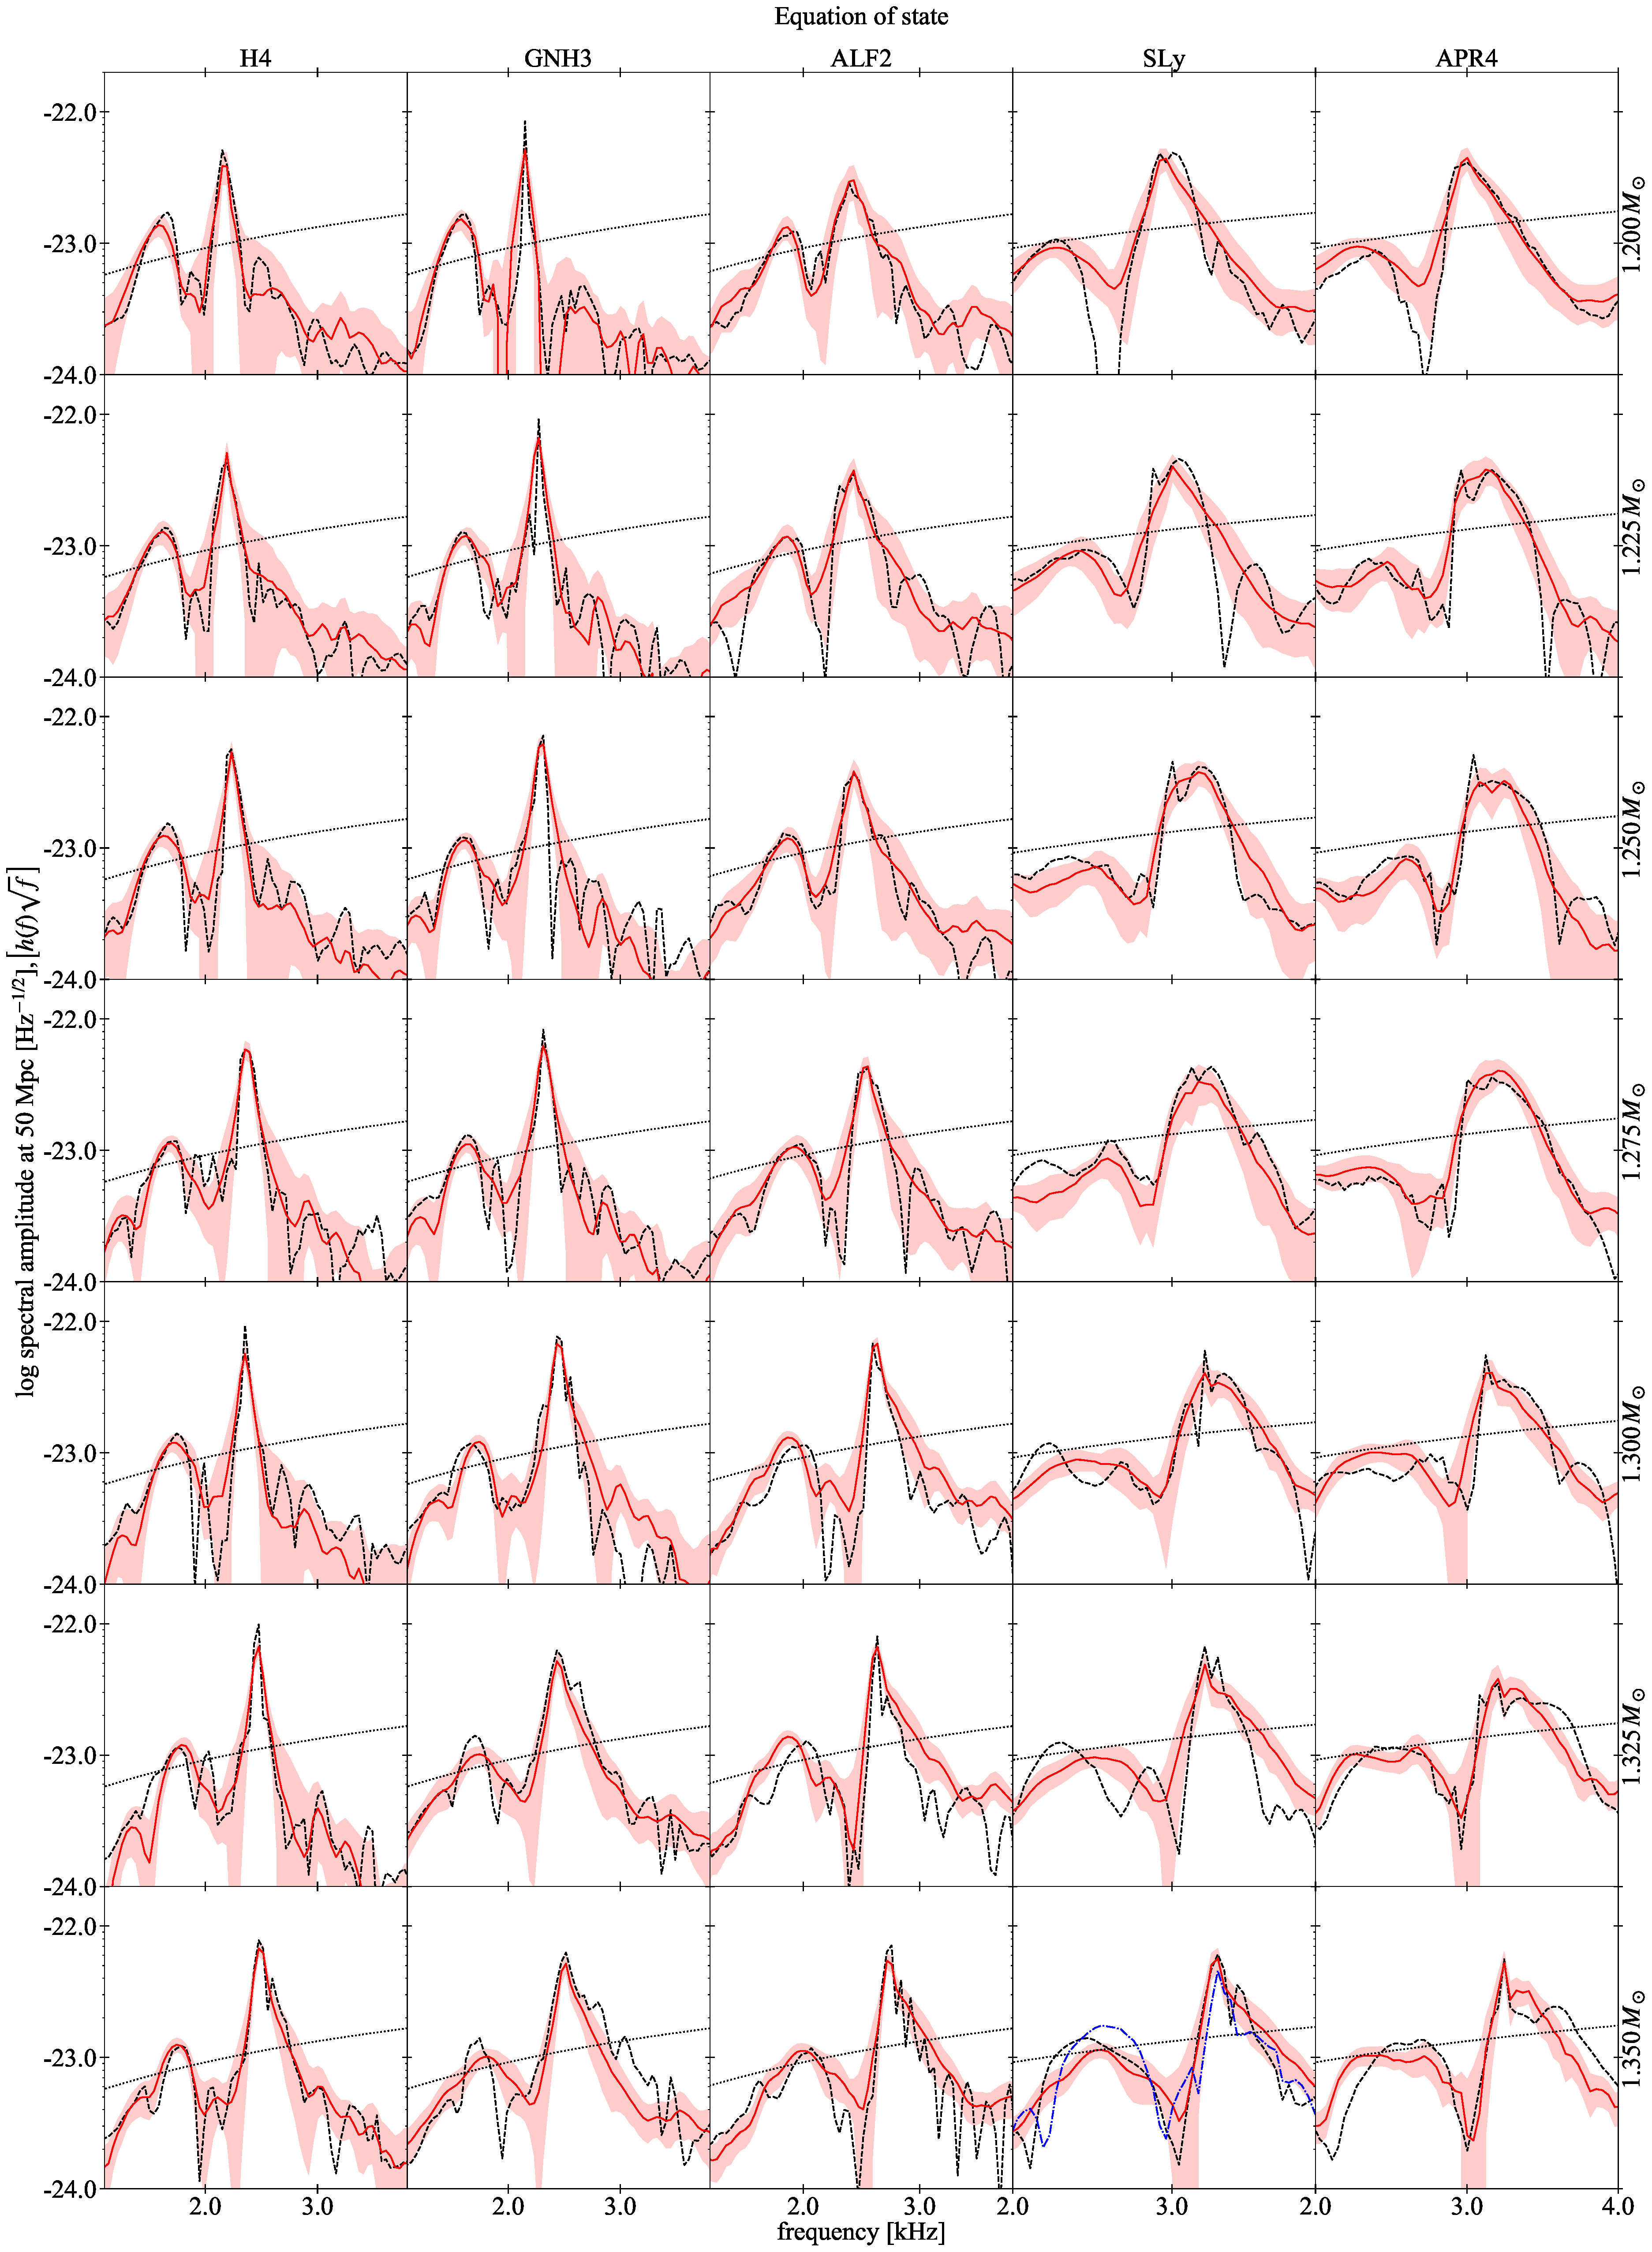
\includegraphics[width=0.94\textwidth]{NewAllMatches35withCoRe.pdf} 
    \caption{ Reconstructed gravitational-wave spectra generated with leave-one-out cross-validation (solid red) and original numerical-relativity spectra~\cite{Rezzolla2016} (dashed black), scaled to a distance of 50 Mpc. Each column represents a different equation of state and each row represents a different neutron star mass, increasing towards the bottom. The one-sigma uncertainty in the spectra is shaded in light red for each prediction.  The Advanced LIGO noise amplitude spectral density (dotted black curve)~\cite{PSD:aLIGO} is shown on all subplots. A numerical-relativity spectrum generated from~\cite{Dietrich2018} is shown (dashed dot blue curve) in the last row (equal mass 1.35\,M$_\odot$) for SLy~\cite{Radice2016} (fourth column) equation of state.}
    \label{fig:GoodPlotsWithWaveformGeneration}
\end{figure*} 
    Simulation of the post-merger phase of binary neutron star mergers is significantly more complicated than the inspiral phase due to the complex physics including shock heating and nonlinear mode coupling. Additional effects, such as neutrino cooling and magnetic fields, are not expected to yield substantial modifications to the locations of the spectral peaks (see e.g. \cite{Giacomazzo2011,Sekiguchi2016,Kawamura2016}), while the role of viscous effects is still a matter of debate \cite{Alford2018}. The accuracy of the resulting simulations can be limited by the trade off between computational constraints and higher resolutions~\cite{Baiotti2017}. This is particularly true for the phase evolution of the post-merger simulations which do not necessarily converge~\cite{Dietrich2018}. However, the power-spectral content is convergent for sufficiently high resolutions (e.g.,~\cite{Takami2015,Dietrich2018}). Our model is representative up to the validity of the numerical-relativity simulations that it is based upon. With this in mind, we wish to encourage further research into numerical-relativity simulations of post-merger remnants to increase the available number of waveforms and to enable further cross-checking between codes.\par
\section{Methodology}
    \sloppy We use 35 numerical-relativity simulations of binary neutron star mergers from~Ref.\cite{Rezzolla2016}, to which we refer to for details on the equations of state employed.  Each simulation consists of non-spinning, equal-mass progenitor neutron stars, with five different equations of state across the simulations.  We train our model on the amplitude  of the characteristic strain spectra, $h_c(f)~=~|\tilde{h}(f)|\sqrt{f}$. Here,  $\tilde{h}(f)$ is the Fourier transform of the plus polarisation of the post-merger gravitational-wave strain, $h_+(t>0)$. The plus and cross polarisations of the simulated gravitational-wave strain have almost identical spectral amplitude and have a phase offset of almost exactly $\pi/2$. We gain no extra information by including the cross polarisation. The merger time, $t=0$, is defined as the time where $h_+^2(t)~+~h_\times^2(t)$ reaches the first maximum. \par
   
    We use a hierarchical model to represent the amplitude spectra. Given a neutron star of mass $M$ and radius $R$, we assume the compactness of a neutron star, $C\equiv M/R$, in the $j$th simulation has a power-law dependence with the mass, $M$, over all equations of state
    \begin{align}
        C_j = \alpha_j M_j^{\beta_j}. 
        \label{eq:Ccalc1}
    \end{align}
        The validity of this model will be determined by how well we can match the numerical-relativity waveforms. The hyperparameters $\{\mathbf{a},\mathbf{b}\}$, and the quadrupolar tidal coupling constant, $\kappa_2^\tau$, determine the values of $\{\alpha,\beta\}$ as follows:
    \begin{align}
        \alpha_j & \sim\mathcal{N}(a_0 + a_1 \kappa_{2,j}^\tau,\sigma_\alpha^2),\label{eq:alphacalc1} \\ 
        \beta_j & \sim\mathcal{N}(b_0 + b_1 \kappa_{2,j}^\tau,\sigma_\beta^2),
        \label{eq:betacalc1}
    \end{align}
        where $\mathcal{N}(\mu,\sigma^2)$ is a Gaussian distribution of mean $\mu$ and variance $\sigma^2$. The quadrupolar tidal coupling constant, $\kappa_2^\tau$, is used due to its importance in the inspiral dynamics~\cite{Damour2010,Read2013,Takami2014,Bernuzzi2015,Takami2015,Rezzolla2016} and its correlation with the location of the main frequency peak of the post-merger spectrum~\cite{Bauswein2012,Takami2014,Bernuzzi2015, Takami2015}.\par
        All spectra in the training set, which excludes the spectrum under test when leave-one-out cross-validation is performed, are used to determine the hyperparameters $\{\mathbf{a},\mathbf{b}\}$ by a least squares fit. The amplitudes for each spectrum are frequency shifted so that the peak frequencies are aligned in a similar way to Refs. \cite{Clark2016postmerger,Bose2018}.  We then fit the aligned spectral amplitudes with a linear model
    \begin{align}
        (h_c)_{i,j} = \boldsymbol{\Theta}_{i}\mathbf{X}_j + \text{noise}, 
        \label{eq:GenerateWaveform1}
    \end{align}
        where the noise is modelled as intrinsic variance, $s_i^2$ for the $i$th frequency bin, $\boldsymbol{\Theta}_i$ is a vector of unknown coefficients,  and $\mathbf{X}_j$ is a design matrix of 
    \begin{align}
        \mathbf{X}_j=[1,\widehat{C}(M_j,\kappa^\tau_{2,j}),\widehat{M}_j,\widehat{\kappa^\tau_{2,}}_{j}]. \label{eq:DesignMatrix1}
    \end{align}
       \noindent The hats indicate the whitened transformations of the neutron star parameters such that $\widehat{\mathbf{x}}\sim~ \mathcal{N}(0,1)=( \mathbf{x}-\mu_x)/\sigma_x$ where $\mu_x$ and $\sigma_x^2$ are the mean and variance of $\mathbf{x}$ respectively. The compactness parameter can be generated from Eqs.(\ref{eq:Ccalc1}-\ref{eq:betacalc1}) after determining the values for $a_0, a_1, b_0$, and $b_1$. Spectra can then be trivially generated given any mass, quadrupolar tidal coupling constant and frequency shift. The frequency shift can be determined from the value of the quadrupolar tidal coupling constant~\cite{Bernuzzi2015,Takami2015}. \par
       We perform leave-one-out cross-validation to test the performance of the model. We do this by excluding the spectrum under test and its associated parameters from the training set. In doing so, the spectra generated during leave-one-out cross-validation represent an extrapolation by the model  and the fitting factors are therefore conservative.
       \par
    \begin{figure}[H]
          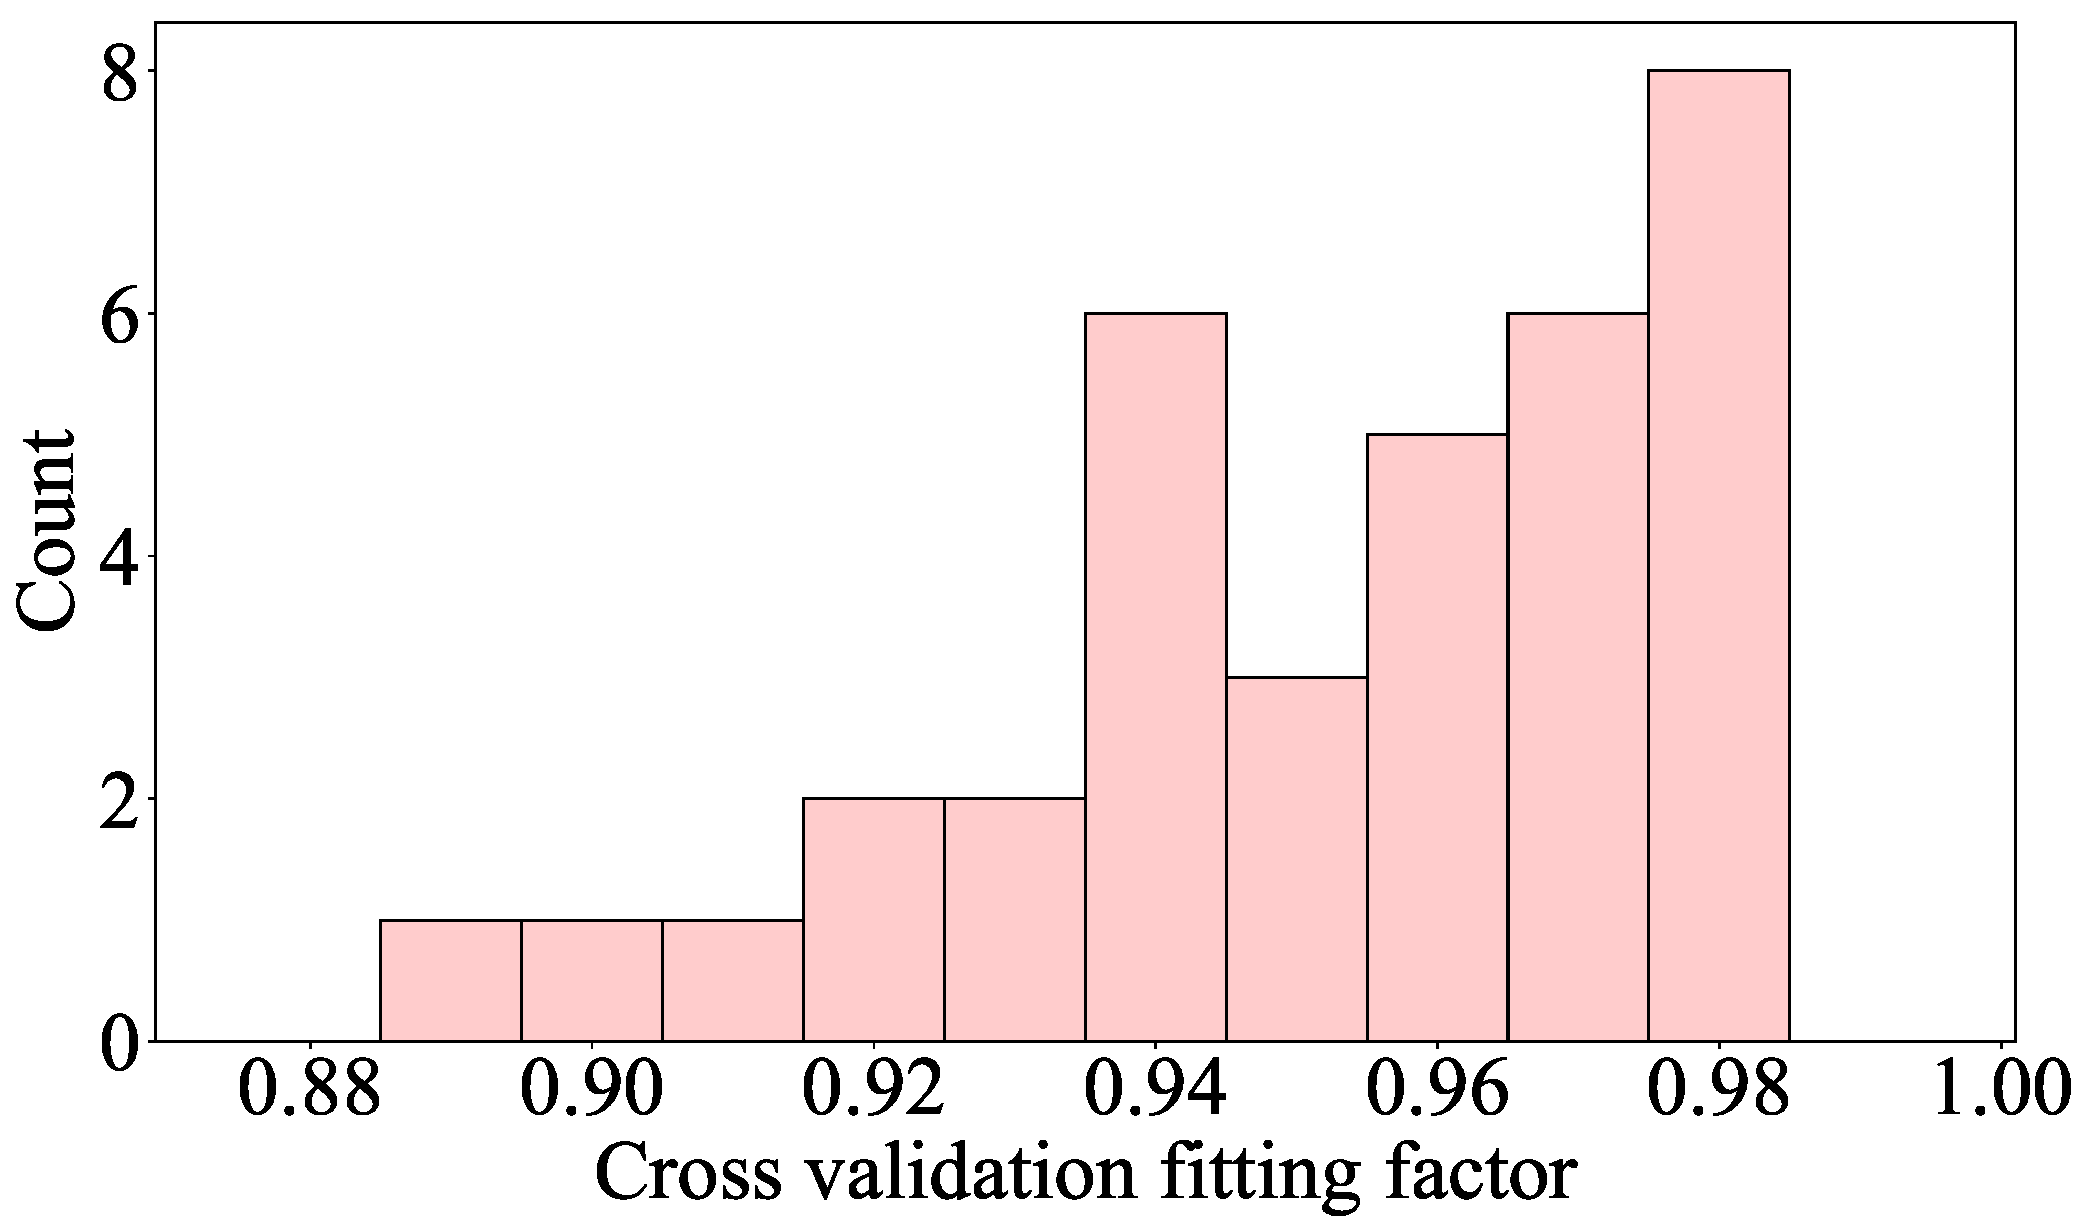
\includegraphics[width=0.99\columnwidth]{newFittingFactorHistogram35.pdf}  
          \caption{Histogram of fitting factors determined by comparing numerical-relativity spectra with spectra generated by our model using leave-one-out cross-validation.}
          \label{fig:FittingFactorsHistogram}
    \end{figure}   
    \begin{figure*}
        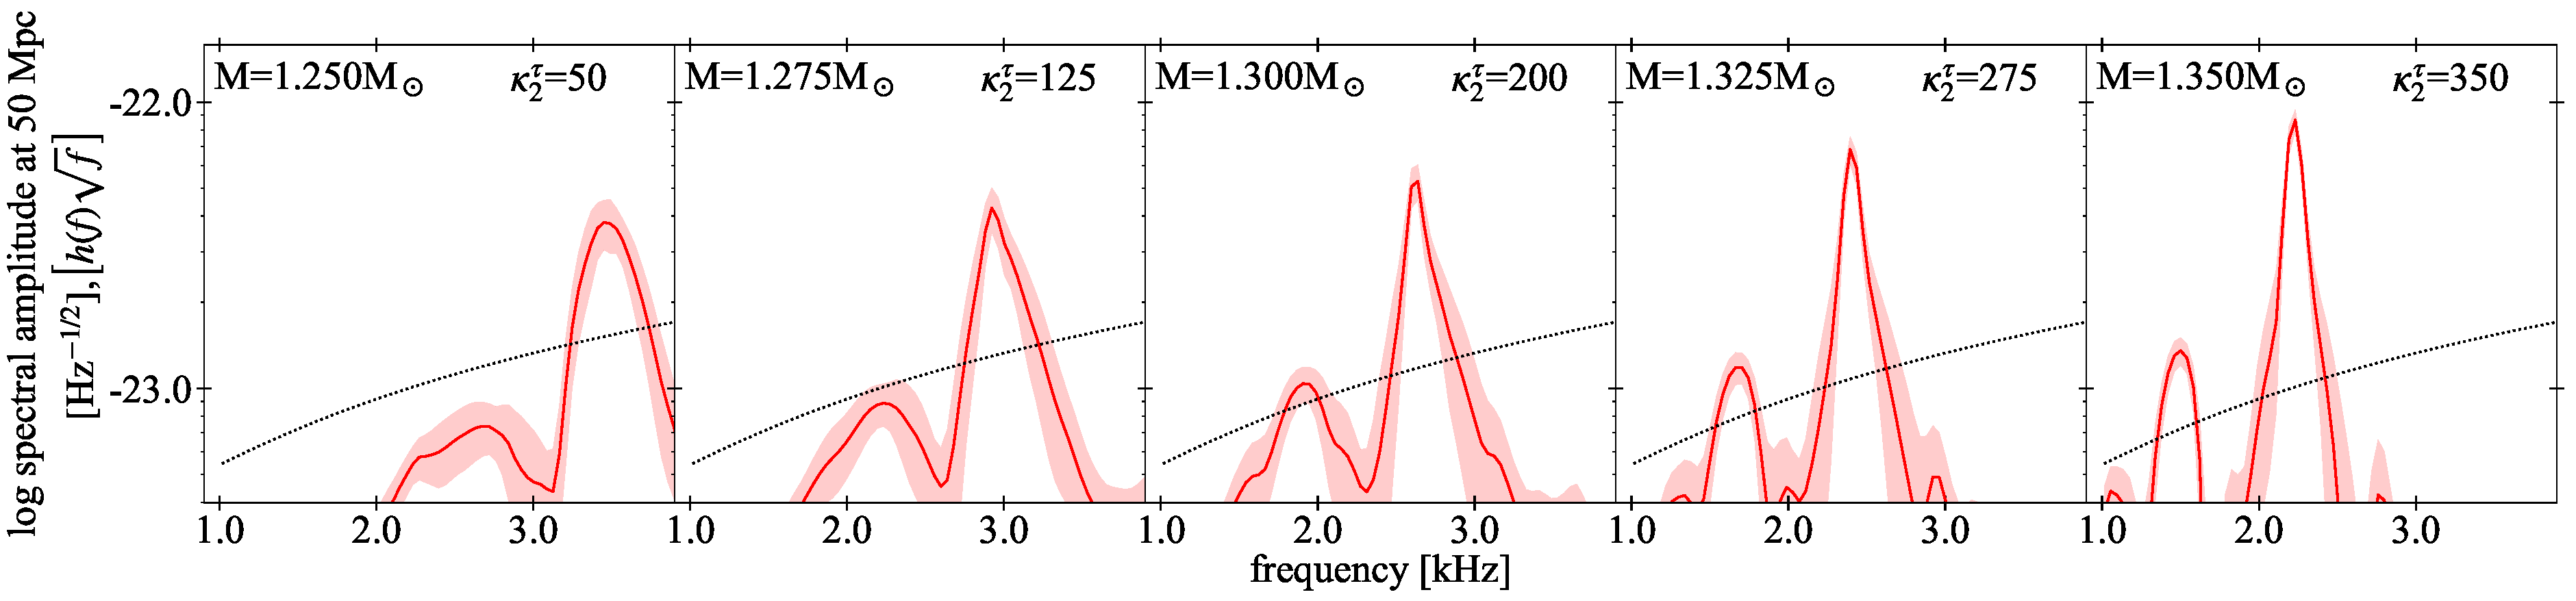
\includegraphics[width=\textwidth]{NewGeneratedWaveforms35.pdf} 
        \caption{ Spectra generated by the model when trained on all the numerical-relativity spectra (red). The uncertainties in the spectra are shown in light red. The Advanced LIGO noise amplitude spectral density (dotted black) is shown on all subplots.}
        \label{fig:GeneratedWaveforms}
    \end{figure*}      
       We perform spectral comparisons using the following noise-weighted fitting factor, or overlap~\cite{Apostolatos95}
        \begin{equation}
        	FF(h_{1},h_{2})\equiv\frac{\left<h_{1}|h_{2}\right>}{\sqrt{\left<h_{1}|h_{1}\right>\left<h_{2}|h_{2}\right>}}.\label{eq:FF1}
        \end{equation}
        Here, the inner product is defined by
        \begin{align}
        	\left<h_1|h_2\right>\equiv4 \int df\frac{|\tilde{h}_1(f)|\ |\tilde{h}_2(f)|}{S_h(f)},
        \end{align}
        where $S_h$ is the noise power spectral  density. Throughout this article we use the \texttt{ZERO\char`_DET\char`_high\char`_P} file from~\cite{PSD:aLIGO} to determine the amplitude of $S_h$. The resultant fitting factor is similar to the standard fitting factor except that it operates on the Fourier amplitude only. A fitting factor of one represents a perfect match. The fitting factor represents the loss incurred to the  optimal signal-to-noise ratio due to mismatch in the model spectra, where the optimal signal-to-noise ratio is given by $\rho_{opt}=\sqrt{	\left<h|h\right>}$.\par
        While it is known that smooth relationships exist between various system properties (e.g., mass, tidal parameters, etc.) and post-merger waveform spectral features~\cite{Bauswein2012,Takami2014,Bernuzzi2015,Takami2015,Bauswein2015,Rezzolla2016}, no such relationships exist for the phase information~(see also~\cite{Messenger2014}). Empirically, while we find good training fits using our model on the spectral content of the waveforms (see below), we are not able to train confidently on the full time series including both phase and amplitude as the phase evolves too quickly between adjacent simulations.  We discuss this in more detail below. \par 

    \section{Results}
        Following the training step, we use Eq.(\ref{eq:GenerateWaveform1}) to generate spectra.  Figure~\ref{fig:GoodPlotsWithWaveformGeneration} shows how well our generated spectra match the original numerical-relativity spectra. The original spectra are shown as dashed black curves, the cross-validation spectra are shown as red curves, and the one-sigma model uncertainty is shown in shaded light red. All spectra are scaled to a distance of 50 Mpc. The Advanced LIGO noise amplitude spectral density is shown as the dotted black curves~\cite{PSD:aLIGO}.  We fit the large-scale structure of the numerical-relativity peaks well with some deviations in the small-scale structure. \par Figure~\ref{fig:FittingFactorsHistogram} shows a histogram of the noise-weighted fitting factor, Eq.(\ref{eq:FF1}), between our cross-validated model prediction and the corresponding numerical-relativity spectra for all tested waveforms. The resulting histogram has a mean of 0.95 with a standard deviation of 0.03. \par
        To place the above results in context, we calculate the nearest neighbour fitting factor of the numerical-relativity spectra. We measure the fitting factor for the spectrum under test against all other spectra, and report the largest fitting factor. We obtain nearest neighbour fitting factors for the numerical-relativity spectra of 0.93 with a standard deviation of 0.05. The fitting factors generated by our model compare favourably with this result. Additionally, our model is capable of generating spectra given the required input parameters, whereas a nearest neighbour interpolation would not be capable of this.\par
           
        As a additional baseline value for comparison, we compare fitting factors between the numerical-relativity spectra used in this paper~\cite{Rezzolla2016}, and those produced with other codes~\cite{Dietrich2018}. Notwithstanding the fact that post-merger waveforms can differ with resolution even when using the same code, we assume that the waveforms have similar truncation errors and compare one set of spectra using equations of state SLy~\cite[THC:0036:R03]{Radice2016} for equal-mass binaries with $M=1.35\,M_\odot$. 
        
        
        The spectrum  for the comparison waveform is plotted (blue dashed dot curve) in the last row and fourth column of Fig.~\ref{fig:GoodPlotsWithWaveformGeneration}, corresponding to the SLy equation of state. This spectrum can be compared to the black dashed waveform from~\cite{Rezzolla2016} in the same panel. While amplitude offsets do not change the fitting factor, differences in the frequency and the shape of the peaks do. The fitting factor between these two waveforms is 0.93. This can be attributed to the difference in the relative shapes of the two main peaks between the simulations in~\cite{Rezzolla2016} and~\cite{Radice2016}.\par
        This comparison indicates that our fitting factors are comparable to the fitting factors between different numerical-relativity codes. We note that numerical simulations are indeed accurate enough for understanding the main structures (e.g., positions of dominant peaks) and their relationship with bulk properties of the remnant. However, our method is limited by the accuracy of the numerical-relativity simulations, which are in turn limited by computational capabilities; we discuss the implications of this below.  \par
        To evaluate how the generated spectra vary, we train on all numerical-relativity spectra and generate a grid of model spectra. We generate spectra at five equally spaced mass and quadrupolar tidal coupling constant values. The mass ranges from $M=1.25\,M_\odot$ to 1.35\,$M_\odot$, and  the quadrupolar tidal coupling constant varies from $\kappa_2^\tau = 50$ to 350. The generated spectra are shown in Fig.~\ref{fig:GeneratedWaveforms} as the red curves,  the one-sigma model uncertainty as light red shading, and the Advanced LIGO noise curve as dotted black. Each of these spectra take a fraction of a second to evaluate. We show these spectra to indicate what we can hope to achieve by implementing these models in full parameter estimation. \par

        In Fig.~\ref{fig:GeneratedFittingFactor} we compare the fitting factor between a spectrum generated with $M=$~1.3\,$M_\odot$, $\kappa_2^\tau=$~100 against spectra generated at other parameter values. We choose $\kappa_2^\tau=$~100 (for an equal-mass system this corresponds to $\Lambda=530$) to be consistent with tidal deformability values, $\Lambda$, determined in \cite{GW170817Detection,Annala2018,Radice2018,Most2018,De2018,GW170817Properties}, under the simplified assumption that $\kappa_2^\tau\approx \frac{3}{16}\Lambda$ (noting that the equality holds for equal-mass progenitors). The location of the reference spectrum is shown with the black cross. This provides the first indication of whether this model could recover the mass and quadrupolar tidal coupling constant when trained on sufficient numerical-relativity simulations. The peak of the contour plot around the reference waveform shows that this model is selective, and may be used for parameter estimation and/or detection in the future. However, this is a task for future work and will require full Bayesian analysis with a noise implementation.
 \begin{figure}[H]
 \begin{center}
    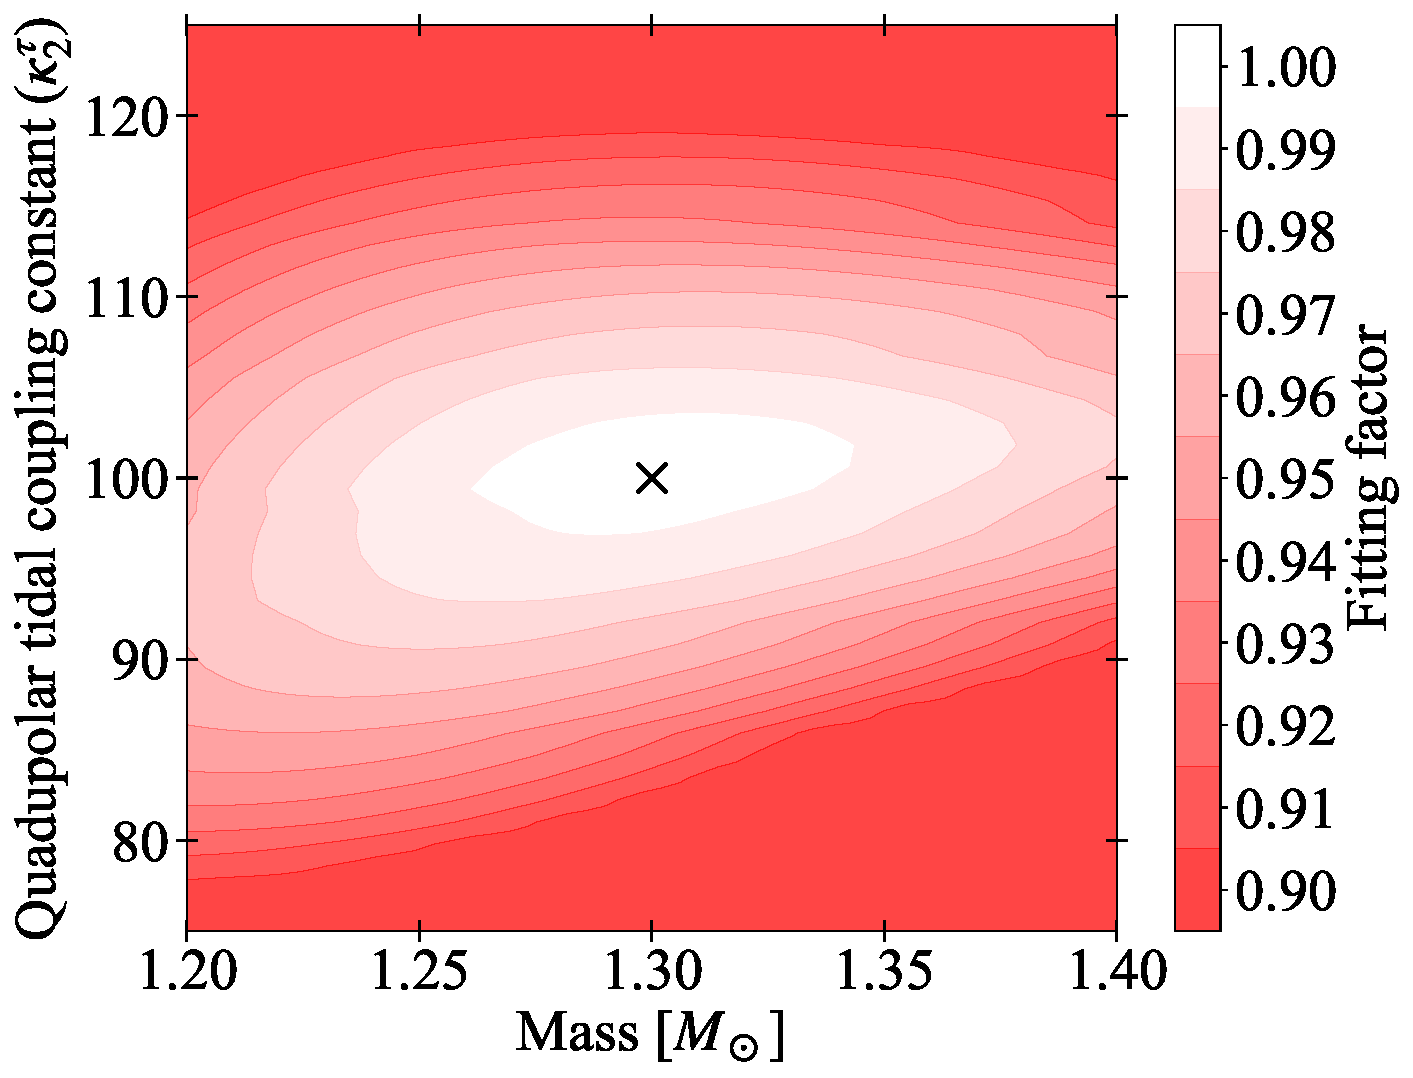
\includegraphics[width=8cm]{NewGeneratedFittingFactor90plus35Kappa100.pdf}
        \caption{Fitting factor between spectra generated using our hierarchical model with 1.30\,$M_{\odot}$ and $\kappa_2^\tau=$100 (black cross), against a grid of mass and quadrupolar tidal coupling constant values.}
        \label{fig:GeneratedFittingFactor}
     
 \end{center}
\end{figure} 
        It is possible that a phase transition may occur in the remnant during the post-merger phase due to an increase in density~(e.g.~\cite{Most2018,Bauswein2018}). This could be detected by comparing the inferred values of the quadrupolar tidal coupling constant from the inspiral and post-merger phases. Simulations that compare hydrodynamic models with and without quark deconfinement show that the presence of quark deconfinement causes no change in the inspiral gravitational-wave signal due to the low densities involved. This is contrasted to the post-merger phase where the densities are greater, leading to a higher proportion of deconfined quarks when modelled, which in turn leads to a change in the post-merger gravitational-wave strain~\cite{Most2018b}. Phase transitions due to quark deconfinement could be detected by training our model on simulations that disallow quark deconfinement. If a post-merger signal was detected that contained the signature of quark-deconfinement then this would result in an inconsistency between the tidal coupling constant inferred from the post-merger gravitational-wave spectra and the inspiral phase. We note that other mechanisms, either physical or arising from errors in the modelling, could also cause such frequency shifts. We leave the exploration of this as future work. \par
    \section{Discussion}
        In this paper, we use a hierarchical model to generate binary neutron star  post-merger spectra by training on spectra generated with numerical-relativity simulations. Our trained model allows us to generate spectra in ${\sim}10^{-4}$ seconds, which significantly reduces the computational effort required to populate a template bank of spectra. We obtain noise-weighted, amplitude-only fitting-factors across all tested spectra, with a mean of 0.95 and a standard deviation of 0.03. This compares favourably to a post-merger fitting factor of 0.93 between different numerical-relativity codes.\par
        Training on the phase of the post-merger spectra will allow fitting factor comparisons with both the amplitude and phase information, as well as the generation of time-based waveforms. In addition, it will provide insight on the number of numerical-relativity simulations required to achieve a complete and accurate database. While obtaining information on the phase evolution is in principle possible, see, e.g.,~\cite{Bose2018}, this also requires a systematic investigation that goes well beyond the scope of this work. Without the phase information, a matched filter search is less sensitive, but it is still possible to design such a search using only the signal amplitudes.
        \par
        Results based on our trained model suggest that the model is selective and could potentially be used in parameter estimation of detected events. If posteriors for the mass and tidal coupling constant are able to be determined, then it is a simple step to calculate the posteriors for the compactness, Eq.(\ref{eq:Ccalc1}), and the radius of the neutron star. This will be confirmed in future work using a Bayesian framework. Parameter estimation of the post-merger spectra could set bounds on the post-merger quadrupolar tidal coupling constant, allowing comparison with the inspiral value. This could determine whether a phase change in the equation of state is present~\cite{Bauswein2018,Most2018b}.\par
        To be valuable in search and parameter-estimation studies, our model must be extended to include individual values of mass, spins, compactness and quadrupolar tidal deformabilities for each progenitor. This paper trained on waveforms with progenitor $\kappa^\tau_2$ values ranging from 50 to 350, and equal-mass progenitors from 1.2 to 1.35\,M$_\odot$. The merger of two progenitors with the same parameters $(C,M,\kappa_2^\tau)$, but different equations of state could produce different output spectra, for example if one equation of state had a lower maximum, non-rotating neutron star mass. This could be a problem for the existing model and an additional input parameter may be needed to remove the degeneracy in the output spectra. This is not necessary for the numerical-relativity simulations that are used in the paper, as there is enough variation in the three parameters to define the output spectra. The model may be also expanded to include simulations with black hole progenitors. In this case the dominant post-merger frequency, corresponding to black hole ring-down, would likely be too high for detection with advanced LIGO. These changes can be introduced given enough numerical-relativity simulations to cover the required ranges of parameter values. The placement of numerical-relativity simulations to enable this is a subject of future work. Our method may eventually provide an additional tool to aid in the detection of short-term post-merger neutron star remnants, supplementing the existing tools~\cite{Klimenko2016,Chatziioannou2017}.
\section*{Acknowledgments}
        PDL is supported through Australian Research Council (ARC) Future Fellowship FT160100112 and ARC Discovery Project DP180103155, ARC is supported in part by the Australian Research Council through Discovery Grant DP160100637. We thank James Clark and Eric Thrane for their feedback.

\end{document}
